\documentclass[border=6pt]{standalone}
\usepackage{tikz}
\usetikzlibrary{arrows.meta,positioning,shapes.geometric,calc}
\begin{document}
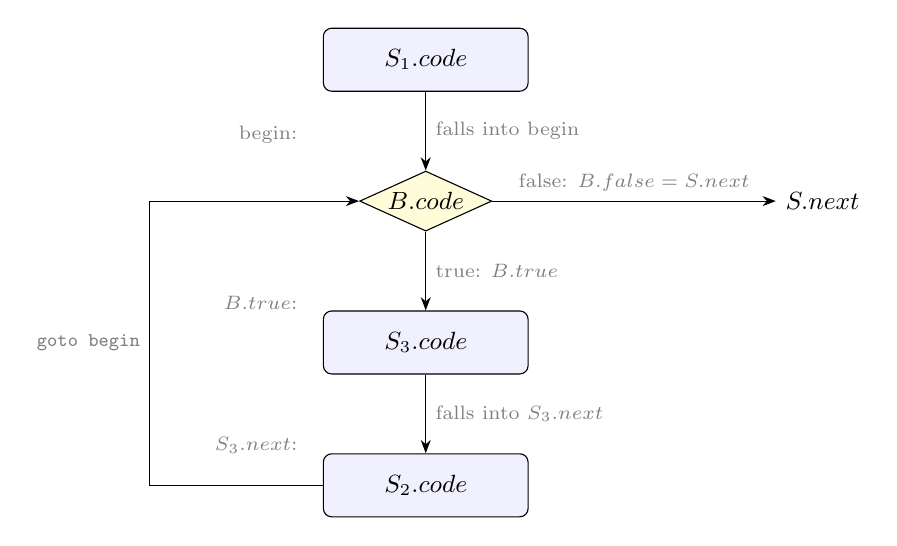
\begin{tikzpicture}[>=Stealth,font=\small,node distance=1.0cm and 2cm,
 blk/.style={draw,rounded corners=3pt,minimum width=2.6cm,minimum height=0.8cm,fill=blue!6},
 cond/.style={draw,diamond,aspect=2.2,inner sep=1pt,fill=yellow!15},
 lab/.style={font=\scriptsize,gray}]
\node[blk] (s1) {$S_1.code$};
\node[cond,below=of s1] (b) {$B.code$};
\node[blk,below=of b] (s3) {$S_3.code$};
\node[blk,below=of s3] (s2) {$S_2.code$};
\node[right=3.6cm of b] (next) {$S.next$};
\draw[->] (s1) -- node[right,lab]{falls into begin} (b);
\draw[->] (b) -- node[right,lab]{true: $B.true$} (s3);
\draw[->] (s3) -- node[right,lab]{falls into $S_3.next$} (s2);
\draw[->] (b) -- node[above,lab]{false: $B.false = S.next$} (next);
\draw[->] (s2.west) -- ++(-2.2,0) |- node[near start,left,lab,align=right]{\texttt{goto begin}} (b.west);
\node[lab,left=0.15cm of b,xshift=-1.3cm] {};
\node[lab,anchor=east] at ($(s1.south west)+(-0.2,-0.55)$) {begin:};
\node[lab,anchor=east] at ($(s3.north west)+(-0.2,0.1)$) {$B.true$:};
\node[lab,anchor=east] at ($(s2.north west)+(-0.2,0.1)$) {$S_3.next$:};
\end{tikzpicture}
\end{document}
